\chapter{Quelque chose à protéger~: Hermione Granger}

\lettrinepara{L}{e} soir passa, le matin vint. Le dernier jour. Le 15 juillet 1992.

\hplettrineextrapara
Les débuts de l'aurore qui annonçaient le lever du soleil illuminaient à peine le ciel. À l'est de Poudlard, là où l'on verrait ce dernier apparaître, par-delà les gradins de Quidditch, une teinte grisâtre rendait à peine visible l'horizon vallonné.

La grande terrasse de pierre où Harry se trouvait était assez grande pour que cette aurore qui naissait derrière les collines fut visible~; il l'avait expressément demandé en décrivant son futur bureau.

Il était pour le moment assis en tailleur sur un coussin. Une brise fraîche parcourait ses mains et pieds nus. Il avait ordonné aux elfes de maison d'amener son trône à paillettes de Général Chaos… puis il leur avait dit de le ranger lorsqu'il avait eu la présence d'esprit de s'inquiéter de l'origine de ses goûts en matière de décorations~; peut-être Voldemort avait-il possédé un trône similaire. Ce qui n'était pas un argument en soi~; ce n'était pas comme si s'asseoir sur un trône à paillettes pour inspecter les terres en contrebas était \emph{immoral} - mais Harry avait décidé de prendre le temps d'y réfléchir. En attendant, de simples coussins suffiraient amplement.

Le nouveau bureau de Harry était situé en dessous, relié au toit par une simple échelle. C'était une grande salle, entourée de quatre fenêtre qui occupaient tout l'espace mural et laissaient passer le soleil~; pour l'instant vide, mis à part quatre chaises et un bureau. Harry avait dit à la directrice ce qu'il voulait, elle avait enfilé le Choixpeau, et elle avait indiqué à Harry quel chemin tortueux parcourir pour se rendre là où il souhaitait être. Si haut que les toits de Poudlard auraient dû s'arrêter avant. Si haut que, vu de l'extérieur, aucune partie du château ne correspondait à l'endroit où Harry se trouvait. Cela avait semblé être une précaution si élémentaire contre les snipers qu'il n'avait vu aucune raison de ne \emph{pas} la prendre.

En revanche, Harry ne savait absolument \emph{où} il était. Si son bureau n'était pas visible de l'extérieur, comment pouvait-il observer cet extérieur~? Comme les photons venus des terres l'atteignaient-ils~? À l'ouest, des étoiles scintillaient encore, bien visibles. Ces photons étaient-ils ceux émis par ces immenses fournaises de plasma situées à d'inimaginables distances~? Ou Harry était-il assis dans une illusion créée par le château de Poudlard~? Ou est-ce que c'était juste 'magique'~? Il fallait qu'il réussisse à faire marcher l'électricité autour de la magie pour pouvoir faire des expériences en plaçant des lasers en bas et en haut.

Et oui, Harry avait maintenant son propre bureau à Poudlard. Il n'avait pas de titre officiel, mais le 'Survivant' était devenu une sorte de meuble de l'école de sorcellerie de Poudlard, terre d'accueil prochaine de la Pierre Philosophe et seul véritable établissement d'enseignement supérieur du monde magique. La sécurité n'était pas encore parfaite, mais le professeur Vector avait mis en place des charmes et runes d'appoint afin de protéger le bureau et le toit des oreilles indiscrètes.

Harry était assis sur son coussin, près du bord du toit de son bureau, et il observait les arbres, les lacs et l'herbe florissante. Loin en bas, des calèches attendaient, pas encore harnachées à des chevaux squelettiques. De petits bateaux jonchaient la côte et se préparaient à transporter de jeunes élèves, lorsque le temps serait venu. Le Poudlard Express était arrivé cette nuit et les wagons et la vieille locomotive attendaient de l'autre côté du lac sud. Tout était prêt pour que les élèves rentrent chez eux après le festin de départ du matin.

Harry regardait le lac et la grande locomotive vieillotte dans laquelle il ne monterait pas. Encore une fois. Cette idée était étrangement triste et inquiétante~; comme s'il commençait déjà à rater des moments de camaraderie avec les \emph{autres élèves de son âge} - même si, après tout, une bonne partie de Harry était née en 1926. Le soir précédent, dans la salle commune de Serdaigle, il avait eut le sentiment que l'écart entre lui et les autres avait bel et bien grandi. Mais cela n'avait peut-être été dû qu'aux questions que Padma Patil et Anthony Goldstein s'étaient posés avec excitation au sujet de la Ressuscitée~; le pépiement de spéculations avait retentit d'un Serdaigle à l'autre. Harry avait connu les réponses, toutes les réponses, mais il n'avait pas pu les dire.

Une partie de Harry voulait monter dans le Poudlard Express puis revenir par le réseau des cheminées. Mais lorsqu'il s'imaginait trouver cinq autres élèves dont il pourrait partager le compartiment et passer les huit heures suivantes à cacher des choses à Neville, Padma, Dean, Tracey ou Lavande… l'idée n'était pas attrayante. Il se sentait obligé de le faire, parce qu'il fallait se \emph{socialiser}, mais il ne \emph{voulait pas} le faire. Il pourrait retrouver les autres au début de l'année prochaine, lorsqu'il y aurait d'autres sujets dont il pourrait parler plus librement.

Il regarda au sud, derrière le lac, en direction de la vieille locomotive, et il pensa au reste de sa vie.

Au Futur.

La prophétie mentionnée par la lettre Dumbledore, où il déchirait les étoiles du ciel… ça, c'était optimiste. Elle avait une interprétation évidente pour tous ceux qui avaient reçu une éducation adéquate. Elle décrivait un futur où l'humanité avait plus ou moins gagné. Ce n'était pas ce qu'il avait le plus souvent en tête en regardant les étoiles, mais d'un point de vue réellement \emph{adulte}, les étoiles constituaient des monceaux immenses de précieuses matières premières qui avaient malheureusement pris feu et devaient être éteints. Si vous pompiez ces énormes réservoirs d'hydrogène et d'hélium, c'était que votre espèce avait réussi à atteindre l'âge adulte.

À moins que la prophétie ait voulu parler d'autre chose. Dumbledore avait peut-être mal interprété les paroles du devin… mais sa lettre avait été formulée comme si une prophétie avait dit que Harry déchirerait \emph{lui-même} les étoiles dans un futur proche. Ce qui pouvait être plus inquiétant, sans être certain, ni même forcément mauvais…

Harry laissa échapper un soupir. Il avait commencé à comprendre, la veille, pendant les longues heures à attendre le sommeil, ce que la dernière lettre de Dumbledore avait vraiment signifié.

Maintenant qu'il comprenait ce qu'il voyait, les événements de l'année scolaire 1991-1992 n'étaient rien moins que terrifiants, capables de vous glacer le sang.

Ce n'était pas juste que Harry avait passé son temps en compagnie de son bon ami Lord Voldemort. Ce n'était même pas le \emph{pire}.

C'était l'image d'une étroite ligne temporelle que Albus Dumbledore avait guidée à travers la petite serrure du destin~; d'un fil de possibilités, fin comme un cheveu, filé dans le chas d'une aiguille.

Les prophéties avaient ordonné à Dumbledore de copier l'intelligence de Tom Jedusor dans le cerveau d'un nourrisson sorcier qui apprendrait ensuite les sciences Moldues. Si c'était \emph{ça}, la meilleure stratégie des devins pour éviter la catastrophe, que pouvait-on en déduire sur la forme probable du Futur~?

Harry pouvait à présent repenser au Serment Inviolable qu'il avait prêté, et deviner que sans ce Serment, le désastre aurait peut-être déjà été rendu inévitable à l'instant où il avait songé à révoquer le Code du Secret Magique. Ce qui suggérait donc que les nombreuses prophéties que Dumbledore avait entendues et dont il avait suivit les instructions étaient parvenues à assurer que Harry et Voldemort entreraient en collision \emph{exactement comme il le fallait}, pour que Voldemort force Harry à prêter ce Serment Inviolable. Que ce Serment avait fait partie de l'étroite serrure du Temps, qu'il avait été l'une des préconditions improbables à la survie des habitants de la Terre.

Un Serment dont le seul but était de protéger tout le monde de la \emph{stupidité} actuelle de Harry.

C'était comme de regarder une vidéo d'un accident de la route que vous aviez évité de justesse. Vous vous souveniez seulement qu'une voiture vous avait raté de quelques centimètres, et la vidéo vous montrait que quelqu'un avait \emph{aussi} lancé un petit caillou qui avait empêché un gigantesque semi-remorque de vous rentrer dedans au même moment~; et que sans ce caillou, vous, votre famille et \emph{toute la planète} auraient été écrasés par le semi-remorque~; dans la métaphore, le semi-remorque représentait votre \emph{profonde inconscience}.

Harry avait été \emph{prévenu}, il avait \emph{su}, sinon le Serment ne l'aurait pas arrêté~; et pourtant il avait \emph{quand même} mal agi, \emph{quand même} failli détruire le monde. Il pouvait y repenser et voir que, oui, l'autre Harry sans Serment aurait eu du mal à accepter de ne pas immédiatement fournir des soins magiques aux Moldus. Même si l'autre Harry avait accepté la présence d'un danger, il l'aurait rationalisée, il aurait essayé d'inventer un moyen astucieux d'éviter le problème, il aurait refusé \emph{d'attendre quelques années}. Et le monde aurait été détruit. En dépit de tous les avertissements, sans le Serment Inviolable, cela n'aurait \emph{pas suffit}.

Un mince fil de Temps, passé par le chas d'une aiguille.

Harry ne savait pas comment réagir à cette révélation. Ce n'était pas le genre de situation pour laquelle l'évolution avait adapté les humains. Il pouvait seulement voir à quel point le désastre avait été proche, à quel point il pourrait s'en \emph{rapprocher} si le Serment se réactivait, et réfléchir…

Réfléchir…

'Je ne veux pas que ça se reproduise' n'était pas une bonne réaction. Il n'avait jamais \emph{voulu} détruire toute la population mondiale. Il n'avait jamais manqué d'instincts protecteurs envers la population sentiente de la Terre~; d'une certaine façon, ces instincts protecteurs avaient \emph{posé problème}. Ce qui manquait à Harry, c'était une vision claire, la volonté d'accepter ce qu'il savait déjà.

Et cette année à faire ami-ami avec le professeur de Défense ne disait pas non plus grand bien de son intellect. Le problème était d'ailleurs quasiment le même. Harry avait soupçonné ou même su certaines choses, mais il ne s'en était jamais rendu conscient. Et il avait donc échoué~; il avait failli mourir.

\emph{Je dois passer à la vitesse supérieure.}

C'était la pensée qui lui avait manquée. Il devait s'améliorer, devenir moins stupide.

\emph{Je dois passer à la vitesse supérieure ou j'échouerai.}

Dumbledore avait détruit tous les enregistrements de la salle des prophéties et avait fait en sorte qu'aucun autre enregistrement ne subsiste. Apparemment, une prophétie avait dit que Harry ne devait pas consulter les autres prophéties. Et la conclusion évidente, qu'elle soit vraie ou pas, était que \emph{même le système des prophéties} ne pouvait pas sauver le monde. Que la victoire nécessitait des plans trop complexes pour être transmis par des devins, ou trop complexes pour être perçus. Si Dumbledore avait pu sauver le monde lui-même, les prophéties auraient probablement indiqué à Dumbledore comment faire. Mais non, elles avaient dit à Dumbledore comment créer les préconditions de l'existence d'une certaine personne~; une personne qui serait peut-être capable de surmonter un défi hors d'atteinte des prophéties elles-mêmes. C'était pour ça que Harry se retrouvait seul, sans devin pour le guider. Il ne deviendrait pas le genre de personne capable de réussir cette tâche inconnue en se bornant à suivre de mystérieux ordres prophétiques à la lettre.

Et pour le moment, Harry James Potter-Evans-Verres était toujours une catastrophe ambulante qui avait besoin d'un Serment Inviolable pour ne pas \emph{immédiatement} rendre inévitable la destruction de la Terre \emph{même après avoir été prévenu}. Et ça datait \emph{d'hier}, juste un jour après avoir failli aider Voldemort à conquérir la planète.

Un passage de Tolkien lui revint à l'esprit, le moment où Frodon, au sommet de la Montagne du Destin, remettait l'anneau~; 'Et Sauron se rendit compte qu'il s'était comporté en \emph{idiot}', ou quelque chose comme ça.

Une immensité séparait le Harry qu'il était aujourd'hui de celui qu'il avait besoin de devenir.

Et il doutait que le temps, l'expérience et la puberté suffiraient. Cela aiderait peut-être. S'il pouvait devenir, comparé à l'enfant qu'il était, ce qu'un adulte était comparé à un enfant de onze ans normal, \emph{peut-être} que cela suffirait à guider le Temps à travers l'étroite serrure…

Il devait réussir à grandir, et aucun sentier battu ne s'étendait devant lui pour le mener à son but.

Il se souvint alors d'une autre fiction, plus obscure que Tolkien~:

\emph{Vous ne pourrez devenir des maîtres qu'en pratiquant les techniques que vous avez apprises, en surmontant des défis, en faisant plein usage des outils qui vous ont été transmis, jusqu'à ce que ceux-ci se brisent entre vos mains et vous laissent au beau milieu de désastres absolus… Je ne peux pas créer de maîtres. Je n'ai jamais su le faire. Allez, et échouez… Vous avez été façonnés pour émerger du désastre déterminés à reconstruire votre Art. Je ne peux pas créer de maîtres, mais sans cet enseignement, vous auriez eu moins de chances d'en devenir. La voie commencera là où l'Art semblera vous faire défaut~; mais en réalité, c'est vous qui aurez fait défaut à votre Art.}

Ce n'était pas qu'il s'était \emph{perdu}, ni que la route vers le bon sens était inaccessible à la science. Mais lire des articles scientifiques n'avait pas \emph{suffit}. Tous les articles de psychologie cognitive sur les bugs du cerveau humains avaient \emph{aidé}, mais ils n'avaient pas \emph{suffit}. Harry n'avait pas réussi à atteindre le niveau de rationalité où l'on commençait à vraiment \emph{réussir}~; il disposait seulement d'un langage pratique pour décrire ses erreurs. Il se rendait à présent compte que le niveau requis était scandaleusement, incroyablement élevé. Il pouvait maintenant repenser à l'année passée et décrire ses errements avec des concepts tels que la 'réflexion motivée'. Cela l'aiderait à l'avenir. C'était mieux que de ne pas savoir quelles erreurs il avait commises. Mais il en fallait plus pour devenir celui qui traverserait l'étroite serrure du Temps, l'adulte dont Dumbledore avait essayé de créer la \emph{possibilité} en suivant les instructions des devins.

\emph{Je dois penser plus vite, grandir plus vite… Suis-je seul, le serais-je~? Est-ce que je fais la même erreur que lors de la première bataille du professeur Quirrell, quand je ne me suis pas rendu compte que Hermione avait des capitaines~? L'erreur que j'ai commise en cachant la sensation funeste à Dumbledore même après m'être rendu compte qu'il n'était probablement ni fou ni méchant~?}

Il aurait été pratique que les écoles moldues enseignent ce genre de leçons, mais ce n'était pas le cas. Peut-être qu'il pourrait recruter Daniel Kahneman, simuler sa mort, lui rendre sa jeunesse par la Pierre et l'envoyer à la recherche de meilleures méthodes d'entraînement…

Harry sortit la Baguette de Sureau de ses robes et regarda à nouveau le bois gris sombre que Dumbledore lui avait transmis. Cette fois, il avait \emph{essayé} de réfléchir plus vite, il avait essayé de compléter le motif que suggéraient la Cape d'Invisibilité et la Pierre de Résurrection. La Cape d'Invisibilité avait le pouvoir légendaire de masquer son porteur et le pouvoir secret de lui permettre de se cacher même de la Mort, incarnée par les Détraqueurs. La Pierre de Résurrection avait le pouvoir légendaire de faire apparaître les morts, et Voldemort l'avait incorporée à son système de Horcruxe pour que son esprit soit libre de se mouvoir. La seconde Relique de la Mort avait été un composant potentiel d'un système d'immortalité véritable que Cadmus Peverell n'avait jamais achevé~; peut-être parce qu'il avait eu un sens moral.

Et il y avait la troisième Relique de la Mort, la Baguette de Sureau d'Antioch Peverell, dont la légende disait qu'elle passait à des sorciers toujours plus puissants et rendait son porteur invincible contre les attaques ordinaires~; c'était sa caractéristique publique…

La Baguette de Sureau avait appartenu à Dumbledore. Il avait essayé d'empêcher la Mort du monde lui-même.

Si la Baguette de Sureau allait toujours au sorcier le plus puissant, c'était pour trouver le meilleur sorcier et le renforcer encore, au cas où l'espèce entière ferait face à une menace~; peut-être était-ce un outil pour vaincre la Mort sous sa forme de destructeur des mondes.

Mais même si un autre pouvoir était cachée dans la Baguette de Sureau, cette pensée n'avait pas suffit à le débloquer. Il avait levé la Baguette de Sureau, il lui avait parlée, il s'était annoncé comme un descendant de Peverell consacré à la quête de sa famille~; il avait promis à la Baguette de Sureau qu'il ferait de son mieux pour protéger le monde de la Mort et poursuivre l'œuvre de Dumbledore. Et la Baguette de Sureau n'avait pas plus répondu à sa main qu'avant, elle avait refusé d'offrir une ellipse à l'histoire. Peut-être Harry devrait-il remporter une première victoire décisive contre la Mort des mondes avant que la Baguette de Sureau ne le reconnaisse~: l'héritier d'Ignotus Peverell avait déjà vaincu l'ombre de la Mort et celui de Cadmus Peverell avait déjà survécu à la Mort de son corps quand leurs Reliques de la Mort respectives avaient révélé leurs secrets.

Il pouvait au moins deviner que, contrairement à la légende, la Baguette de Sureau ne contenait pas de 'crin de Sombral'. Il avait vu des Sombraux~: c'étaient des chevaux squelettiques à la peau soyeuse, sans crinière, aux têtes semblables à des crânes, sans touffe de poils sur leur queue osseuse. Il ignorait ce qui se trouvait réellement dans la Baguette de Sureau et il n'avait pas non plus pu trouver où que ce soit le symbole du cercle, du triangle et de ligne qui aurait dû y être inscrit.

"J'imagine," murmura-t-il à la Baguette de Sureau, "que tu ne pourrais pas juste me répondre~?"

Aucune réponse ne vint de la baguette à pommeaux~; seulement le sentiment d'une gloire et d'une puissance contenue qui l'observait avec scepticisme.

Il soupira et remit la baguette la plus puissante du monde dans ses robes d'écolier. Il finirait par trouver~; pourvu que ce soit à temps.

Peut-être qu'il trouverait encore plus vite si quelqu'un l'aidait dans ses recherches.

Il avait en partie conscience - non, il devait arrêter d'avoir \emph{en partie conscience} des choses et commencer à juste en être conscient - il était explicitement, consciemment conscient du fait que ses ruminations au sujet du Futur servaient avant tout à le distraire de l'arrivée imminente de Hermione Granger. Qui s'était réveillée en parfaite santé à Sainte Mangouste et avait transplané avec le professeur Flitwick jusqu'à Poudlard. Qui avait dit à ce dernier qu'elle devait immédiatement parler à Harry Potter. Harry avait trouvé une note de lui-même à son intention en se réveillant plus tard dans la matinée, le soleil déjà haut au-dessus du dortoir de Serdaigle. Il l'avait lue et était retourné dans le temps avant l'heure matinale où Hermione Granger arriverait.

\emph{Elle ne sera pas en colère contre moi.}

\emph{…}

\emph{Sérieusement. Hermione n'est pas comme ça. Peut-être qu'elle l'était au début de l'année, mais elle se connaît trop bien pour ça maintenant.}

\emph{…}

\emph{Comment ça, '…'~? Si tu as quelque chose à dire, voix intérieure, dis-le~! On essaie d'être plus conscient de nos pensées, tu te rappelles~?}

\later

Le ciel était devenu entièrement gris et l'aube était presque dénuée de soleil quand Harry entendit le bruit de pas venir de l'échelle qui donnait sur son nouveau bureau. Il se leva en hâte et épousseta ses robes, puis, réalisant ce qu'il faisait, cessa ses gestes nerveux. Bon sang, il venait de vaincre Voldemort, pas besoin d'être aussi mal à l'aise.

La tête et les boucles châtain de la jeune sorcière apparurent par l'ouverture et pivotèrent. Elle monta encore, comme si elle courrait sur les barreaux, comme si elle avançait le long d'un chemin qui se trouvait être vertical~; S'il avait cligné des yeux au mauvais moment, Harry aurait pu manquer la façon dont l'une de ses chaussures toucha brièvement le dernier barreau avant qu'elle ne bondisse et n'atterrisse avec légèreté sur le toit.

\emph{Hermione.} Les lèvres de Harry bougèrent, mais il ne fit aucun bruit.

Il avait voulu lui dire quelque chose, mais il avait oublié.

Quinze secondes s'écoulèrent peut-être avant que Hermione Granger ne parle. Elle portait un uniforme à bordures bleues et la cravate bleue et bronze de sa Maison.

"Harry," dit Hermione Granger, une voix si terriblement familière que Harry en pleura presque, "avant que je ne te pose toutes mes questions, je voudrais commencer par te dire merci, merci beaucoup pour, euh, ce que tu as fait, quoi que ce soit. Sincèrement. Merci."

"Hermione", dit Harry, et il déglutit. Il avait imaginé commencer par \emph{Ais-je la permission de te prendre dans mes bras}, mais cela lui semblait impossible à dire. "Bon retour. Attends un instant, je vais lancer quelques sorts contre les oreilles indiscrètes." Harry sortit la Baguette de Sureau de ses robes, prit un livre dans sa bourse qu'il ouvrit à un marque-page et prononça avec précaution~: "\emph{Hominum Revelio}", ainsi que deux autres sortilèges de sécurité récemment appris et qu'il était devenu à peine capable de lancer grâce à la Baguette de Sureau. Ce n'était pas grand chose, mais c'était marginalement mieux que de seulement compter sur le professeur Vector.

"Tu as la baguette de Dumbledore," dit Hermione. Elle avait parlé d'une voix étouffée et pourtant aussi puissante qu'une avalanche. "Et tu peux l'utiliser pour lancer des sortilèges de quatrième année~?"

Harry hocha la tête et nota mentalement de ne pas montrer ça à n'importe qui. "Est-ce que je peux te prendre dans mes bras~?"

Hermione s'avança vivement vers lui~; ses mouvements étaient étrangement plus rapides, plus gracieux qu'auparavant. Une pureté semblait émaner d'eux, et elle lui rappela à quel point elle avait eu l'air paisible, endormie sur l'autel de Voldemort…

Le souvenir lui revint comme une tonne de plomb~; ou au moins comme un kilo de plomb.

Et il serra Hermione dans ses bras, ressentit la \emph{vie} qui se dégageait d'elle. Il voulut pleurer, mais se retint, car il ne savait pas si c'était seulement son aura qui l'affectait.

Autour de lui, les bras de Hermione étaient très doux. Ils exerçaient une pression particulièrement légère, comme si elle faisait attention à ne pas briser son corps comme un vieux cure-dents.

"Donc," dit Hermione une fois que Harry l'eut laissée échapper à son étreinte. Son jeune visage semblait à la fois très sérieux, très pur et très innocent. "Je n'ai pas dit aux Aurors que tu étais là, ni que c'est le professeur Quirrell, pas Tu-Sais-Qui, qui a tué tous les Mangemorts. Le professeur Flitwick ne les a laissé me donner qu'une seule goutte de Veritaserum, donc je n'ai pas été obligée de parler. J'ai juste dit que je me souvenais seulement du troll."

"Ah," dit Harry. Il s'était retrouvé à regarder le nez de Hermione plutôt que ses yeux. "Et tu penses qu'il s'est passé quoi, exactement~?"

"Eh bien," dit Hermione Granger tout en réfléchissant, "je me suis fait manger par un troll, ce que j'aimerais franchement ne plus jamais avoir à vivre, et puis il y a eu un grand \emph{bang} et mes jambes étaient revenues, j'étais allongée sur un autel de pierre au milieu d'un cimetière, la nuit, dans une forêt sombre que je n'avais jamais vue, avec les mains arrachées de quelqu'un serrées autour de ma gorge. Alors tu vois, Harry Potter, en me retrouvant dans une situation aussi bizarre, glauque et effrayante, je n'allais pas refaire la même erreur que la dernière fois avec Tracey. J'ai su \emph{tout de suite} que c'était toi."

Harry hocha la tête. "Bien vu."

"Je t'ai appelé, mais tu n'as pas répondu," dit Hermione. "Je me suis redressée et l'une des mains en sang a glissé sur ma chemise en laissant des bouts de chair derrière elle. Mais je n'ai pas crié, même en me rendant compte que j'étais entourée de têtes et de corps et que l'odeur que je sentais, c'était du sang." Hermione se tut et inspira profondément. "J'ai vu les masques de crânes et j'ai compris que les gens morts avaient été des Mangemorts. J'ai tout de suite su que le professeur de Défense avait été là avec toi et les avait tous tués, mais je n'ai pas remarqué le corps du professeur Quirrell. Je ne me suis pas rendu compte que c'était lui même en regardant le professeur Flitwick inspecter le corps. Il avait l'air… différent, une fois mort." Sa voix devint plus faible. Elle avait un air humble que Harry ne se souvenait pas avoir déjà observé chez elle. "Ils ont dit que David Monroe s'était sacrifié pour me faire revenir comme ta mère s'était sacrifiée pour toi, pour que le Seigneur des Ténèbres explose à nouveau en essayant de me toucher. Je suis \emph{assez} sûre que ce n'est pas tout à fait vrai… mais j'ai eu beaucoup de mauvaises pensées au sujet de notre professeur de Défense, et elles étaient injuste."

"Euh," dit Harry.

Hermione hocha solennellement la tête et joint ses mains, comme en signe de pénitence. "Je sais que tu es probablement trop gentil pour me dire ce que tu as tout à fait le droit de me dire, alors je vais le dire pour toi, Harry. Tu avais raison au sujet du professeur Quirrell, et j'avais tort. Tu me l'as dit. David Monroe était un peu obscur et très Serpentard, et c'était puéril de ma part de croire que ça voulait dire qu'il était méchant."

"Ah…" répondit Harry. Il eut beaucoup de mal à répondre. "En fait, le reste du monde ne le sait pas encore, même pas la directrice, mais tu avais cent-douze pour cent raison sur sa méchanceté, et je me souviendrai à l'avenir que même si 'obscur' et 'maléfique' ne sont pas synonymes, il y a une bonne grosse corrélation statistique entre les deux."

"Ah," dit Hermione, et elle redevint silencieuse.

"Tu ne me dis pas que tu me l'avais bien dit~?" demanda Harry. Son modèle mental de Hermione hurlait~: JE TE L'AVAIS BIEN DIT~! JE TE L'AVAIS DIT OU PAS~? OUI OU NON~? LE PROFESSEUR QUIRRELL EST MÉCHAAAAAAANT, JE L'AI DIT, MAIS TU \emph{NE M'AS PAS ÉCOUTÉE~!}

La véritable Hermione se contenta de secouer la tête. "Je sais que tu avais beaucoup d'affection pour lui," dit-elle doucement. "Puisque j'avais raison en fin de compte… je savais que tu souffrirais probablement beaucoup en apprenant qu'il était méchant, et que ce ne serait pas le bon moment pour te dire que je t'avais prévenu. Enfin, c'est ce que j'ai décidé il y a plusieurs mois en pensant à un moment comme celui-ci."

\emph{Merci, Hermione Granger.} Harry était quand même heureux d'entendre ça, sans quoi il n'aurait pas eu l'impression de parler à Hermione.

"Donc, M. Potter," dit Hermione Granger en tapant ses doigts sur sa hanche. "Quand la médicomage m'a fait une prise de sang, la douleur est partie immédiatement, et quand j'ai essuyé la petite goutte de sang sur mon bras, je n'ai pas pu trouver le trou de l'aiguille. J'ai tordu un barreau de mon lit sans forcer, et même si je n'ai pas encore pu vérifier, j'ai l'impression que je peux courir \emph{très} vite. Mes ongles sont d'un blanc nacré alors que je ne me rappelle pas les avoir peints. Mes dents aussi, et comme je suis fille de dentistes, ça m'inquiète. Alors ce n'est pas que je suis ingrate, mais qu'est-ce que tu as fait, exactement~?"

"Euh," dit Harry. "Et je suppose que tu te demandes aussi pourquoi une aura de pureté et d'innocence émane de toi~?"

"Une QUOI~?"

"Ce n'était pas mon idée. Franchement." Harry avait une toute petite voix. "Ne me tue pas, s'il te plaît."

Hermione Granger regarda ses ongles de près en louchant presque. "Harry, est-ce que tu… Enfin, si j'irradie de l'innocence, si je suis rapide et gracieuse, si mes dents sont d'un blanc nacré… Est-ce que mes ongles sont en \emph{alicorne}~?"

"Alicorne~?"

"Ça veut dire corne de licorne, Harry Potter." Elle avait l'air d'essayer de mordiller un ongle sans grand succès. "Donc je suppose que quand on fait revenir une fille d'entre les morts, elle devient une… Comment disait Daphné… Une Princesse Licorne Scintillante~?"

"Ce n'est pas exactement ce qui s'est passé," répondit Harry, mais elle n'était vraiment pas tombée loin.

Hermione enleva son doigt de sa bouche et fronça les sourcils. "Je ne peux pas le mordre non plus. Harry Potter, as-tu pensé aux problèmes que je vais avoir maintenant que je suis littéralement incapable de me couper les ongles des mains et des pieds~?"

"Les jumeaux Weasley devraient avoir une épée magique adéquate," répondit Harry.

"Je pense," dit Hermione Granger d'un ton ferme, "que j'aimerais connaître toute l'histoire, Harry Potter. Parce que vous connaissant, le professeur Quirrell et toi, je dirais qu'il y a un \emph{plan} derrière tout ça."

Harry inspira profondément. Puis il souffla. "Désolé mais… C'est top secret. Je pourrais te le dire si tu avais étudié l'Occlumancie mais… Le veux-tu~?"

"Est-ce que je veux étudier l'Occlumancie~?" dit Hermione d'un air légèrement surpris. "Ce n'est pas au moins niveau sixième année~?"

"Je la pratique," dit Harry. "J'ai commencé avec un avantage, mais je pense que ça ne change pas grand chose sur le long terme. Enfin, je suis sûr que tu pourrais apprendre le calcul différentiel en t'y mettant sérieusement, quel que soit l'âge auquel les Moldus l'apprennent. La question est, euh." Harry avait du mal à contrôler sa respiration. "La question est de savoir si tu veux encore faire… ce genre de choses."

Hermione se retourna et observa le ciel qui s'éclaircissait à l'est. "Tu veux dire," dit-elle doucement, "si je veux encore être une héroïne maintenant que ça m'a déjà valu une mort horrible."

Harry hocha la tête puis dit "Oui" parce que Hermione ne le regardait pas. Le mot resta comme bloqué dans sa gorge.

"J'ai réfléchi à ça," dit Hermione. "C'était effectivement une mort particulièrement atroce et douloureuse."

"J'ai, euh. J'ai mis en place certaines choses \emph{juste au cas où} tu voudrais toujours être une héroïne. J'ai eu une brève opportunité de le faire mais pas le temps de te demander ton avis, et je ne pouvais pas te laisser me voir parce que je m'attendais à ce qu'on te donne du Veritaserum plus tard. Mais si ça ne te plaît pas, je peux en défaire la majeure partie et tu peux juste ignorer le reste."

Hermione hocha la tête. Elle avait un air distant. "Comme de faire croire à tout le monde que j'ai… Harry, est-ce que j'ai \emph{vraiment} fait quoi que ce soit à Tu-Sais-Qui~?"

"Non, c'était moi, mais ne le dis à personne, s'il te plaît. Pour info, la fois où le Survivant a prétendument vaincu Voldemort, la nuit de Halloween 1981, on la doit à Dumbledore, et il a laissé tout le monde croire que c'était moi. Donc maintenant j'ai vaincu un Seigneur des Ténèbres une fois et j'en ai eu les lauriers une fois. J'imagine que tout finit par s'équilibrer."

Hermione continua de contempler l'Est. "Ça me dérange un peu," dit-elle au bout d'un moment. "Ces gens qui pensent que j'ai vaincu Voldemort alors que je n'ai rien fait du tout… ah, mais c'est ce que tu as déjà vécu."

"Ouais. Désolé de t'infliger ça. J'étais… j'imagine que j'essayais de te donner une identité à part dans l'esprit des gens. Je n'ai eu qu'une seule chance de le faire et tout s'est fait de façon assez \emph{hâtive} et… je me suis rendu compte ensuite que j'aurais peut-être dû m'abstenir, mais il était trop tard." Harry s'éclaircit la gorge. "Mais, euh. Si tu veux agir à la hauteur de l'image de la Ressuscitée, euh. J'ai peut-être une idée pour toi. Quelque chose tu pourras faire très bientôt, si tu veux."

Hermione Granger le \emph{regardait}.

"Mais tu n'est pas \emph{obligée}~!" s'empressa-t-il de répondre. "Tu peux juste ignorer tout ça et être la meilleure élève de Serdaigle~! Si c'est ce que tu préfères."

"Est-ce que tu fais de la psychologie inversée sur moi, Harry Potter~?"

"Non~! Honnêtement~!" Harry inspira profondément. "J'\emph{essaie} de ne pas décider de ta vie à a ta place. Hier, j'ai cru voir… j'ai cru voir ce que l'avenir te réservait… mais ensuite je me suis rappelé du temps que j'ai passé à faire l'idiot cette année. J'ai pensé à certaines choses que Dumbledore m'a dites. Je me suis rendu compte que ce n'était vraiment pas à moi de choisir. Que tu pouvais faire ce que tu voulais de ta vie, et qu'avant tout, ça devait être ta décision. Peut-être qu'après tout ça, tu ne veux \emph{pas} devenir une héroïne, peut-être que tu veux devenir une grande chercheuse en magie, parce que c'est ce que tu es vraiment, peu importe la composition de tes ongles. Ou tu pourrais aller à l'institut des sorcières de Salem aux États-Unis au lieu d'aller à Poudlard. Je ne vais pas te mentir en te disant que ça me plairait, mais c'est vraiment à toi de voir." Harry se tourna vers l'horizon et fit un large geste de la main, comme pour désigner le monde qui s'étendait devant Poudlard. "Tu peux aller \emph{n'importe où}. Tu peux faire \emph{ce que tu veux}. Si tu en as envie, je peux te transformer en un triton sexagénaire. Je suis sérieux."

Hermione hocha lentement la tête. "Je me demande comment tu ferais ça, mais je ne veux pas qu'on fasse des choses \emph{pour} moi."

Harry soupira. "Je comprends. euh…" Il hésita. "Je pense… si ça peut t'aider… dans mon cas, on a fait \emph{beaucoup} de choses pour moi. Surtout Dumbledore, mais le professeur Quirrell aussi. Peut-être qu'il faut mériter le pouvoir de choisir son destin."

"Dis-moi, ça a l'air fort sage," dit Hermione. "Mes parents paieront mes cours d'université pour que j'obtienne un travail plus tard. Le professeur Quirrell m'a ressuscitée sous la forme d'une Princesse Licorne Scintillante, tu as dit je nous avais débarrassés du Seigneur des Ténèbres. C'est pareil, en fait."

"Je \emph{suis} désolé," dit Harry. "Je sais que j'aurais dû faire les choses autrement mais… je n'avais pas beaucoup de temps, j'étais épuisé, je ne réfléchissais pas clairement…"

"Je te suis reconnaissante, Harry," dit Hermione d'une voix adoucie. "Tu t'en veux trop. Ne prends pas mes moqueries au sérieux. Je ne veux pas être le genre de fille qui ressuscite et commence à se plaindre de ses nouveaux superpouvoirs et du type de nacre de ses ongles en alicorne." Elle s'était à nouveau détournée et contemplait l'Est. "Mais, Harry Potter… si je décide effectivement qu'une mort horrible ne suffit pas à me faire reconsidérer mes choix… non pas que ce soit le cas… qu'est-ce qui se passe ensuite~?"

"Je fais de mon mieux pour te soutenir dans tes choix," dit Harry d'un ton ferme. "Quels qu'ils soient."

"J'imagine que tu as déjà une quête pour moi. Une jolie quête sans danger, sans la moindre chance qu'il m'arrive quoi que ce soit."

Harry se frotta les yeux. Il pouvait entendre la voix d'Albus Dumbledore en lui. \emph{Pardonne-moi, Hermione Granger…} "Je suis désolé, Hermione. Si tu choisis cette voix je vais être obligé de faire mon Dumbledore et de te cacher certaines choses. De te manipuler, mais pas pour longtemps. Je pense que tu pourrais faire quelque chose, quelque chose de concret, à la hauteur de l'image que les gens ont de la Ressuscitée… je pense que tu pourrais même avoir un destin particulier… mais je ne fais que deviner, j'en sais beaucoup moins que Dumbledore. Est-ce que tu es prête à risquer la vie que tu viens de récupérer~?"

Hermione se tourna vers lui, les yeux écarquillés sous l'effet de la surprise. "\emph{Risquer ma vie~?}"

Harry ne hocha pas la tête, car cela aurait été mentir. "Es-tu prête à le faire~?" préféra-t-il répondre. "La quête que je pense faire partie de ta destinée… et non, je ne connais aucune prophétie, je ne fais que deviner… cette quête nécessite que tu descendes presque littéralement en enfer."

"Je pensais…" dit Hermione. Elle semblait incertaine. "J'étais quasiment sûre qu'après ça, toi et le professeur McGonagall ne me… tu sais… ne me laisseraient pas faire quoi que ce soit de dangereux."

Harry ne répondit pas~; les bons points non mérités qu'il recevait le faisaient se sentir coupable. Hermione avait de fait un modèle particulièrement fidèle de lui, et si Hermione n'avait pas eu de Horcruxe, la surface de Vénus aurait atteint des températures proches du zéro absolu avant que Harry ne fasse une proposition pareille.

"Sur une échelle de zéro à cent, à quel point cette image de descente aux enfers est-elle littérale~?" dit Hermione. Elle avait l'air un peu inquiète.

Harry effectua un équilibrage mental, se remémora Azkaban. "Je dirais environ quatre-vingt sept~?"

"Ça ressemble à une quête pour plus tard, quand je serais plus âgée, Harry. Il y a une différence entre l'héroïsme et la folie."

Harry secoua la tête. "Je ne pense pas que le risque serait très différent," répondit-il, éludant ainsi la nature exacte du risque, "et c'est le genre de chose qui, quitte à être faite, gagne à être faite au plus tôt."

"Et mes parents n'ont pas voix au chapitre~?" demanda Hermione.

Harry haussa les épaules. "Nous savons tous les deux ce qu'ils diraient, et tu peux le prendre en compte si ça te chante. Euh, j'ai demandé à ce que les docteurs Granger ne soient pas informés de ton retour. Ils l'apprendront quand tu reviendras de ta mission, si tu l'acceptes. Ça m'a l'air plus bienveillant envers leurs nerfs, de leur donner une franche bonne surprise plutôt que de les laisser s'inquiéter de… de trucs."

"Que c'est attentionné," dit Hermione. "J'apprécie que tu t'inquiètes pour eux. Est-ce que je pourrais y réfléchir pendant quelques minutes~?"

Harry fit un geste vers le coussin qu'il avait placé face au sien, et Hermione s'y installa avec grâce et fluidité, face au rebord du toit, émanant toujours la même tranquillité. Il fallait vraiment régler ça, peut-être en payant quelqu'un pour qu'il invente une potion anti-pureté.

"Est-ce que je dois décider sans connaître la mission~?" demanda-t-elle.

"Certainement \emph{pas}," répondit Harry en réfléchissant à une conversation similaire avant son propre voyage vers Azkaban. "C'est le genre de chose que tu dois choisir librement. Ça fait partie intégrante de la mission. Si tu me dis que tu veux toujours être une héroïne, je te dirai la mission plus tard - quand tu auras eu le temps de manger, de parler à des gens, de récupérer un peu - et tu décideras à ce moment là si tu as envie de le faire. Et on vérifiera à l'avance que ton retour à la vie te permet bien de lancer le sortilège que les sorciers ordinaires croient être impossible."

Hermione hocha la tête et redevint silencieuse.

Le ciel s'était encore éclairci lorsqu'elle parla à nouveau.

"J'ai peur," dit Hermione, presque dans un souffle. "Pas de mourir à nouveau, ou pas \emph{seulement} de ça. J'ai peur de ne pas être à la hauteur. J'ai eu ma chance de vaincre un troll, et je suis juste morte…"

"C'était un troll renforcé par Voldemort, transformé en arme, et en plus il avait saboté tout ton équipement magique."

"Je suis morte. Et toi tu as réussi à tuer le troll, je crois que je m'en souviens, il ne t'a même pas ralenti." Hermione ne pleurait pas, pas une larme ne coulait sur ses joues, elle regardait simplement le ciel toujours plus lumineux, là où le soleil allait apparaître. "Et ensuite tu m'as ressuscitée sous la forme d'une Princesse Licorne Scintillante. Je \emph{sais} que je n'aurais pas pu faire ça. J'ai peur de ne \emph{jamais} en être capable, quoi que les gens pensent de moi."

"C'est ce genre de choses qui fait partie intégrante de ton aventure, je pense…" il s'interrompit. "Pardon, je ne devrais pas essayer d'influencer ta décision."

"Non," murmura-t-elle, les yeux toujours braqués vers les collines en contrebas. Elle éleva la voix. "Non, Harry, je veux entendre ce que tu as à dire."

"D'accord. Euh. Je crois que c'est ça ton \emph{point de départ}. Tout ce qui s'est passé jusqu'à aujourd'hui… ça te met là où j'étais en septembre, dans la position d'un enfant prodige qui trouve un nouveau palier vers lequel se hisser. Si tu ne te comparais pas à moi, à…" \emph{mes motifs cognitifs adultes copiés de Tom Jedusor} "… mon côté obscur… tu serais l'étoile montante de Serdaigle, celle qui a organisé un groupe de combat contre les brutes, est resté saine d'esprit face à l'assaut de Voldemort, à seulement douze ans. J'ai vérifié~: tu as eu de meilleures notes que Dumbledore n'en avait en \emph{première} année." \emph{Sans compter la note de Défense, c'était juste Voldemort en train de faire son Voldemort.} "Maintenant, tu as quelques pouvoirs et une réputation à tenir, et le monde est sur le point de te faire travailler dur. C'est là où tout \emph{commence} pour toi, comme ça a commencé pour moi. Ne te sous-estime pas." Et Harry se tut soudain, parce qu'il était en train de la \emph{persuader}. Il avait au moins réussi à s'arrêter avant de lui demander \emph{qui} pourrait être un héros, si même elle ne pouvait pas en être un.

"Tu sais," dit Hermione, toujours face à l'horizon, "j'ai eu une conversation de ce genre avec le professeur Quirrell, sur le fait d'être un héros. Il était contre, bien sûr. Mais à part ça, ça ressemble beaucoup à sa façon d'argumenter."

Harry garda ses lèvres cousues. Il était difficiler de laisser les gens faire leurs propres choix, parce que c'était prendre le risque qu'ils fassent le \emph{mauvais}. Mais il fallait quand même le faire.

Hermione parla avec précaution. Les liserets bleus de son uniforme de Poudlard paraissaient plus clairs contre ses robes noires, contre le ciel soudain illuminé autour d'eux~; à l'ouest, plus aucune étoile n'était visible. "Le professeur Quirrell m'a dit qu'il avait été un héros autrefois. Mais que les gens ne l'aidaient pas assez, et qu'il avait donc abandonné et qu'il était parti faire quelque chose de plus intéressant. Je lui ai dit que ça avait été mal de sa part de faire ça - en fait, j'ai dit que c'était horrible. Il a dit que oui, qu'il était peut-être une personne horrible, mais que cela en disait peut-être long sur ceux qui n'avaient même jamais essayé d'être des héros. Est-ce qu'ils étaient encore pire que lui~? Et je n'ai pas su quoi lui répondre. Enfin, c'est mal de dire que seuls les héros à la Gryffondor sont des gens bien - même si je pense que du point de vue du professeur Quirrell, c'était plutôt que seuls les gens très ambitieux avaient le droit de respirer. Et je n'étais pas d'accord avec ça. Mais ça m'avait aussi l'air mal \emph{d'arrêter} d'être un héros, de tout abandonner comme il l'avait fait. Alors je ne lui ai pas répondu et je suis passée pour une idiote. Mais maintenant, je sais ce que j'aurais dû lui dire."

Harry contrôla sa respiration.

Hermione se releva et se tourna vers Harry. "Je ne vais plus essayer d'être une héroïne," dit Hermione Granger, le ciel de l'Est toujours plus radieux autour d'elle. "Je n'aurais jamais dû penser comme ça. Les gens font juste ce qu'ils peuvent, quand ils le peuvent. Et il y en a aussi d'autres qui ne font même pas de leur mieux, et oui, c'est mal. Je ne vais plus jamais essayer d'être une héroïne. Je ne vais plus \emph{penser} en termes héroïques, si j'y arrive. Mais je ferai aussi tout ce qui est en mon pouvoir - ou presque tout, je suis humaine, après tout." Harry n'avait jamais compris ce qui était mystérieux dans le sourire de la Joconde, mais il sentait que, s'il avait pu photographier le sourire à la fois joyeux et résigné de Hermione, il aurait pu le contempler pendant des heures sans comprendre, et que Dumbledore, lui, l'aurait immédiatement compris. "Je ne veux pas tirer d'enseignement de cette leçon. Je \emph{vais} être stupide. Je vais continuer de faire presque tout ce qui est en mon pouvoir, ou au moins \emph{une partie} de ce qui est en mon pouvoir… bon, tu vois ce que je veux dire. Même si ça veut dire que je vais à nouveau risquer ma vie, tant que ça vaut le coup et que ce n'est pas… \emph{vraiment} stupide. C'est ma réponse." Avec un air résolu, Hermione prit une profonde inspiration. "Alors, qu'est-ce que je peux faire~?"

Harry avait une boule dans la gorge. Il mit la main dans sa bourse et, incapable de parler, il traça les lettres C-A-P-E et sortit le tissu fuligineux de la Cape d'Invisibilité avant de l'offrir à Hermione pour la dernière fois. Harry dut forcer les mots à sortir~: "C'est la Véritable Cape d'Invisibilité," dit-il en chuchotant presque, "la Relique de la Mort transmise par Ignotus Peverell à ses descendants puis aux Potters. Et maintenant, à toi…"

"Harry~!" s'exclama Hermione. Elle plaqua ses bras contre sa poitrine comme pour se protéger de l'attaque du cadeau. "Tu n'as pas à faire ça~!"

"\emph{Si}, il le faut. J'ai quitté le chemin qui me permet d'être un héros, je ne pourrai plus jamais prendre le risque de partir à l'aventure. Et toi… tu peux." Il leva la main qui ne tenait pas la Cape et s'essuya les yeux. "Je pense qu'elle a été faite pour toi. Pour la personne que tu vas devenir. \emph{Une arme pour combattre la Mort lorsqu'elle revêt la forme de l'ombre du désespoir qui s'abat sur les humains et draine leurs espoirs futurs~; je crois que c'est elle que tu combattras, sous d'autres formes encore que celle des Détraqueurs…}"Je ne te prête pas ma Cape, je te la donne, Hermione Jean Granger. Protège-la à jamais."

Hermione tendit lentement la main et saisit la Cape avec l'air d'essayer elle aussi de ne pas pleurer. "Merci," chuchota-t-elle. "Je pense… même si j'en ai fini avec l'héroïsme… que tu as toujours été mon vieux sorcier mystérieux."

"Et je pense," dit Harry, sa gorge à moitié bloquée, "que même si tu rejettes cette façon de penser, tu as toujours été destinée à devenir l'héroïne, depuis le début de cette histoire." \emph{Que doit devenir Hermione Granger, quelle forme adulte devra-t-elle adopter pour pouvoir traverser l'étroite serrure du Temps~? J'ignore la réponse à cette question, pas plus que je ne peux imaginer mon moi adulte. Mais ses prochains pas semblent plus clairs que les miens…}

Harry laissa partir la Cape, et elle passa d'une main à l'autre.

"Elle chante," dit Hermione. "Elle me chante une chanson." Elle leva une main et s'essuya les yeux. "Je n'arrive pas à croire que tu aies fait ça, Harry."

Son autre main sortit de sa bourse, munie d'une longue chaîne en or d'où pendait une coquille en or. "Et c'est ta machine à voyager dans le temps personnelle."

Il y eut un instant de silence pendant lequel la planète Terre poursuivit son orbite.

"Quoi~?" dit Hermione.

"Ils appellent ça un Retourneur de Temps. Poudlard en a un stock à distribuer à certains élèves et j'en ai eu un au début de l'année pour arranger mon rythme du sommeil. Il permet à l'utilisateur de remonter dans le temps par incréments d'une heure, six au maximum. Cela m'a permis d'étudier pendant six heures de plus tous les jours. Et de disparaître du cours de potions, et ainsi de suite. Ne t'en fais pas, un Retourneur de Temps ne peut pas changer l'histoire ou créer des paradoxes qui détruisent l'univers."

"Tu restais à mon niveau en cours en étudiant six heures de plus par jour grâce à une \emph{machine à voyager dans le temps}." Hermione Granger paraissait avoir du mal à digérer l'idée.

Harry prit un air interloqué. "Ça te surprend~?"

Hermione tendit la main et prit le collier en or. "J'imagine que ça ne devrait pas, je suis une sorcière," répondit-elle. Elle avait un ton un peu acerbe. Elle plaça la chaîne autour de son cou et le sablier dans sa chemise. "Mais maintenant, je suis particulièrement contente d'être restée à ton niveau, alors merci."

Harry s'éclaircit la gorge. "Et aussi, puisque Voldemort a décimé la Maison Monroe et qu'ensuite, tu as prétendument vengé cette Maison en tuant Voldemort, je me suis arrangé pour que Amelia Bones fasse passer une loi en vitesse auprès de ce qui reste du Magenmagot disant Granger est maintenant une Maison Noble d'Angleterre."

"Pardon~?" dit Hermione.

"Ce qui fait de toi la seule héritière d'une Maison Noble, ce qui signifie que tu n'as qu'à passer le BUSE pour obtenir ta majorité, ce qu'on fera à la fin de l'été pour avoir un peu de temps pour étudier. Si ça te convient, bien sûr."

Hermione Granger émit le genre de son aigu qui, venu d'un appareil moins organique, aurait indiqué un dysfonctionnement mécanique. "J'ai deux mois pour réviser mon BUSE~?"

"Hermione, c'est un test fait pour que la plupart des élèves de quinze ans le réussissent. Des élèves de quinze ans \emph{ordinaires}. On aura une note passable avec un niveau de troisième année si on apprend les bons sortilèges, et c'est tout ce qu'il nous faut pour être majeurs. Mais tu devras accepter de n'avoir qu'une mention Assez Bien plutôt que tes habituelles félicitations du jury."

Les bruits aigus qui émanaient de Hermione montèrent encore d'un cran.

"Voilà ta baguette," dit Harry en la sortant de sa bourse. "Et ta bourse en peau de Moke~; après ta mort, je me suis assuré que tout y soit au complet." Harry sortit cette bourse d'une poche de ses robes, car l'idée de placer un \emph{sac sans fond} dans un autre \emph{sac sans fond} l'inquiétait, même si c'était censé être sans danger du moment que les deux sacs avaient été fabriqués selon les normes de sécurité habituelles.

Hermione reprit sa baguette puis sa bourse, et elle parvint à rendre ces gestes gracieux malgré le tremblement de ses doigts.

"Voyons voir, quoi d'autre… le serment que tu as prêté à la maison Potter ne t'engageait que 'jusqu'au jour de ta mort', donc tu en es libérée. Et juste après ta mort, je me suis arrangé pour que les Malfoys déclarent publiquement que tu étais innocente de tous les chefs d'accusations."

"Merci beaucoup, Harry," répondit-elle. "C'était particulièrement gentil de ta part, et de leur part à eux aussi, je suppose." Elle n'arrêtait pas de passer ses doigts dans ses boucles châtain, comme si, en arrangeant ses cheveux, elle pourrait restaurer sa santé mentale.

"Enfin et surtout, j'ai dit aux gobelins de commencer à construire une chambre forte à Gringotts, au nom de Granger," continua-t-il. "Je n'y ai pas mis d'argent parce que je pouvais attendre de te demander ton avis. Mais si tu vas être une superhéroïne redresseuse de torts, ça pourrait être utile que les gens te perçoivent comme appartenant à d'une certaine élite, et, euh, je pense que ça sera utile qu'ils sachent que tu as les moyens de t'offrir des avocats. Je peux mettre autant d'or que tu veux dans ta chambre forte, puisque je me suis retrouvé en possession de la Pierre Philosophale après le meurtre de Nicolas Flamel par Voldemort."

"Je pense que je devrais m'évanouir," dit Hermione d'une voix flûtée, "mais mes superpouvoirs m'en empêchent, et d'ailleurs, \emph{pourquoi} est-ce que j'ai des superpouvoirs~?"

"Si ça te va, tes cours d'Occlumancie commenceront mercredi avec M. Bester, il pourra te voir une fois par jour. Jusque là, je pense qu'il vaut mieux que la véritable origine de tes pouvoirs ne puisse pas être révélée par un simple Legilimens qui t'aurait regardée dans les yeux. Enfin, bien sûr, il y a une explication magique normale, ce n'est pas super-supernaturel, mais les gens ont tendance à vouer un culte à leur ignorance, et je pense que la Ressuscitée produira un meilleur effet si elle est entourée d'une aura de mystère. Quand tu pourras empêcher M. Bester d'entrer dans ton esprit et que tu pourras résister au Veritaserum, je te dirai tout, je te le promets, y compris des secrets que tu ne peux dire à personne d'autre."

"Ça s'annonce génial," dit Hermione Granger. "Je suis impatiente."

"Mais tu vas devoir prêter un Serment Inviolable par lequel tu t'engages à ne rien faire qui risque de détruire le monde avant que je ne te dise les parties les plus dangereuses de l'histoire. En fait, je ne peux littéralement pas te le dire sans ça, parce que j'ai prêté un Serment Inviolable moi aussi. Ça te va~?"

"Bien sûr," dit Hermione. "Pourquoi est-ce que ça ne m'irait pas~? De toute façon, je ne veux pas détruire le monde."

"Est-ce que tu as besoin de t'asseoir encore~?" dit Harry, alarmé par le balancement léger de Hermione, comme au rythme des mots qui étaient prononcés.

Hermione Granger prit quelques inspirations profondes. "Non, je pète la forme," dit-elle. "Est-ce qu'il y a autre chose que je dois savoir~?"

"C'est tout. J'ai fini, pour l'instant en tout cas." Harry s'interrompit. "Je comprends que tu veuilles te débrouiller seule et qu'on ne fasse pas les choses à ta place. C'est juste que… Tu vas devenir une véritable héroïne, et ce ne serait pas raisonnable de ma part de ne pas te donner tous les avantages possibles…"

"Je comprends tout à fait," dit Hermione. "Maintenant que j'ai perdu un vrai combat et que je suis morte. Je ne comprenais pas, mais maintenant, si." Une brise agita les cheveux châtain et les robes de Hermione, lui donnant un air encore plus paisible, lorsqu'elle leva une main et serra le poing. "Si je fais ça, autant que je le fasse \emph{bien}. On va mesurer ma force, la hauteur de mes sauts, voir si mes ongles peuvent tuer un Moremplis comme une vraie corne de licorne le peut, et je devrais m'entraîner à utiliser ma vitesse pour éviter les sortilèges qui ne doivent vraiment pas m'atteindre et… et tu pourrais peut-être trouver un Auror pour m'entraîner, celui qui a entraîné Susan Bones, par exemple." Hermione souriait à nouveau, avec dans ses yeux une étrange lueur qui aurait profondément interloqué Dumbledore et que Harry saisit tout de suite, avec une légère appréhension. "Oh~! Et je veux porter des armes Moldues, cachées peut-être, pour que personne ne sache que j'en ai. J'ai pensé à des grenades incendiaires quand je me suis battue contre le troll, mais je n'ai pas pu les Métamorphoser assez vite, même quand j'ai arrêté de m'inquiéter au sujet du règlement de l'école."

"J'ai l'impression," dit Harry en faisant de son mieux pour imiter l'accent Écossais du professeur McGonagall, "que je ne peux pas vous laisser faire ça."

"Oh c'est beaucoup, BEAUCOUP trop tard, Harry Potter. Par exemple, est-ce que je pourrais avoir un bazooka~? Le lance-missile, pas le chewing-gum~? Je parie qu'ils ne s'attendront pas à ce qu'une jeune fille ait \emph{ça}, surtout si j'émane une aura d'innocence et de pureté."

"Bon," dit Harry d'un ton calme, "\emph{maintenant} tu commences à m'effrayer."

Hermione arrêta de tenir en équilibre sur la pointe de son pied gauche, un bras tendu dans un sens et sa jambe droite tendue dans l'autre, comme une danseuse de ballet. "Ah bon~? Je commençais juste à me demander ce que je pouvais faire qu'une escouade ministérielle d'élite ne pourrait pas faire. Ils ont des balais très rapides et des sortilèges plus puissants que les miens." Elle abaissa gracieusement sa jambe. "Parce que maintenant que je peux essayer des trucs sans risquer d'être vue, je commence à penser que j'aime vraiment, \emph{vraiment} avoir des superpouvoirs. Mais je ne vois toujours pas comment je pourrais gagner un combat que le professeur Flitwick perdrait, sauf si j'attaque le mage noir par surprise."

\emph{Tu peux prendre des risques qu'aucun autre ne devrait prendre et réessayer en sachant ce qui t'a tuée. Tu peux faire des essais avec de nouveaux sortilèges, plus qu'aucun autre, en sachant que tu ne mourras pas.} Mais Harry ne pouvait rien en dire pour le moment, alors il se contenta de dire~: "Je pense que tu peux plus penser à l'avenir qu'à ce que tu peux faire maintenant."

Hermione sauta très haut, frappa trois fois des talons pendant sa descente, et atterrit sur ses pointes de pied dans une posture parfaite. "Mais tu as dit que je pouvais faire quelque chose tout de suite. Ou est-ce que c'était juste un test~?"

"\emph{Ça}, c'est un cas particulier," dit Harry, et il sentit le froid de la matinée rafraîchir sa peau. Il avait de moins en moins envie de dire à super-Hermione que son supplice l'amènerait en face de son pire cauchemar, au sens propre, dans des circonstances où sa force physique serait inutile.

Hermione hocha la tête et jeta un coup d'œil vers l'Est. Elle alla rapidement jusqu'au bord du toit, les pieds presque au-dessus du vide. Harry s'y rendit aussi et s'assit en tailleurs, plus loin du bord.

Au loin, un dégradé de rouge s'élevait au-dessus des collines à l'Est de Poudlard.

Regarder le début du lever de soleil redonna sa bonne humeur à Harry. Tant que le soleil était dans le ciel, tout allait bien, en un sens. Par exemple, cela voulait dire qu'il ne l'avait pas encore détruit.

"Donc," dit Hermione. Sa voix monta d'un cran. "En parlant du futur, Harry. J'ai eu le temps de réfléchir à beaucoup de choses pendant que j'attendais à Sainte Mangouste et… c'est peut-être bête, mais je veux toujours connaître la réponse à une certaine question. Tu te rappelle de notre dernière conversation~? Je veux dire, avant …~?"

"Quoi~?" répondit immédiatement Harry.

"Oh…" dit Hermione. "C'était il y a deux mois pour toi… j'imagine que tu ne t'en souviens pas."

Et il se souvint.

"Ne t'en fais pas!" dit Hermione quand un étrange son étranglé sortit de la gorge de Harry. "Je promet que, quoi que tu dises, je n'éclaterai pas en sanglots, je ne m'enfuirai pas, et je ne me ferai pas à nouveau manger par un troll~! Je sais que ça fait moins de deux jours pour moi, mais je pense que la mort a rendu beaucoup de mes préoccupations moins importantes, comparées à ce que j'ai traversé~!"

"Oh," dit Harry d'une voix à présent aiguë. "Je suppose que c'est une bonne façon d'exploiter un traumatisme majeur."

"Sauf que, tu vois, je me pose \emph{toujours} la question, Harry, parce que pour moi nous ne nous sommes pas parlé il y a longtemps, et nous n'avons pas fini de parler, et j'admets que c'était ma faute si j'ai perdu le contrôle de mes émotions et que je me suis ensuite faite manger par un troll, ce que je ne compte certainement pas réitérer. Je me suis dit que je devrais te rassurer~: ça ne se passera pas comme ça à chaque fois que tu diras une bêtise à une fille." Toujours assise, Hermione gigotait, de gauche à droite, d'avant en arrière. "Mais, eh bien, même les gens qui \emph{sont} amoureux ne font littéralement pas un centième de ce que tu as fait pour moi. Alors, M. Harry James Potter-Evans-Verres, si ce n'est pas de l'amour, je veux savoir ce que je représente à tes yeux exactement. Tu ne me l'as jamais dit."

"C'est une bonne question," dit Harry en essayant de contrôler une panique naissante. "Ça t'embête si j'y réfléchis un moment~?"

Peu à peu, le cercle violemment lumineux devint de plus en plus visible, par-delà les collines.

Le soleil avait à moitié dépassé les collines quand Harry dit~: "Hermione, as-tu déjà formulé des hypothèses pour expliquer mon mystérieux côté obscur~?"

"Seulement les hypothèses évidentes," dit Hermione, en balançant un peu ses jambes au-dessus du rebord du toit. "J'ai pensé que Tu-Sais-Qui avait peut-être envoyé la magie qui créé les fantômes en mourant à côté de toi et avait imprimé une partie de lui dans ton cerveau plutôt que dans le plancher. Mais ça m'a toujours eut l'air bizarre, comme une explication intelligente qui n'est pas \emph{vraie} pour autant, et elle a encore moins de sens si Tu-Sais-Qui n'est pas vraiment mort cette nuit-là."

"Pas mal," dit Harry. "Gardons ce scénario pour le moment." Son rationaliste interne se tapait la tête contre les murs. Comment avait-il pu ne pas penser à des hypothèses comme celle-ci. Ce n'était pas vrai, mais c'était \emph{raisonnable}, et Harry n'avait jamais construit de modèle causal concret comme celui-ci, seulement émis l'idée d'une vague connexion.

Hermione hocha la tête. "Tu le sais probablement déjà, mais je préfère le dire~: Tu n'es pas Voldemort, Harry."

"Je sais. C'est \emph{ça}, ce que tu représentes pour moi." Harry inspira. Il avait encore du mal à le dire. "Voldemort… n'était pas quelqu'un d'heureux. Je ne sais pas s'il a été heureux un seul jour de sa vie." \emph{Il n'a jamais pu lancer le Patronus.} "C'est en partie pour ça que ses motifs cognitifs ne m'ont pas dominé~: mon côté obscur n'a jamais été agréable, il ne déclenchait pas de renforcement positif. Mon amitié avec toi, ça veut dire que ma vie n'a pas à ressembler à celle de Voldemort. Et j'étais assez solitaire à Poudlard, sauf que je ne m'en suis pas rendu compte tout de suite, alors… ouais. Peut-être que te ramener d'entre les morts était plus important pour moi que ça ne l'aurait été pour un autre garçon de mon âge. Mais je maintient que ma décision était le résultat d'un raisonnement moral parfaitement normal et que si les autres se soucient moins de leurs amis, c'est leur problème, pas le mien."

"Je vois," dit Hermione avec douceur. Elle hésita. "Harry, ne le prends pas mal, mais ça me dérange un peu. C'est une grosse responsabilité que je n'ai pas choisie, et je ne pense pas que ce soit sain de mettre ça sur les épaules d'une seule personne."

Harry hocha la tête. "Je sais. Mais ça va plus loin. Il y a une prophétie qui a dit que j'allais vaincre Voldemort…"

"Une \emph{prophétie}~? Il y a une \emph{prophétie} sur toi~? Vraiment, Harry~?"

"Oui, je sais. Bref, une partie de la prophétie disait~: 'Et le Seigneur des Ténèbres le marquera comme son égal, mais il aura un pouvoir que le Seigneur des Ténèbres ignore.' Est-ce que tu pourrais deviner ce que c'est~?"

"Hmmm," dit Hermione. Ses doigts tapèrent pensivement la pierre du toit. "Ton mystérieux côté obscur est la marque de Vous-Savez-Qui qui fait de toi son égal. Le pouvoir qu'il ignore… c'est la méthode scientifique, non~?"

Harry secoua la tête. "C'est ce que je pensais aussi… que ce serait la science Moldue, ou les méthodes de la rationalité. Mais…" il expira. Le soleil était maintenant loin au-dessus des collines. Il était gêné, mais il fallait le dire. "Le professeur Rogue, qui a entendu la prophétie le premier - oui, je sais - le professeur Rogue a dit que ça ne pourrait pas être seulement la science, que le 'pouvoir que le Seigneur des Ténèbres ignore' devait être plus étranger à Voldemort que ça. Même si je pense en termes de rationalité, eh bien, il s'avère que Voldemort," \emph{enfin, le professeur Quirrell,} l'idée rendait encore Harry malade, "aurait été capable d'apprendre les méthodes de la rationalité s'il avait lu les mêmes articles scientifiques que moi. Sauf peut-être une seule chose…" Harry inspira. "À la fin, lors de ma confrontation finale avec Voldemort, il a menacé de mettre mes parents et mes amis à Azkaban. À moins que je ne trouve des secrets intéressants à lui révéler, une personne sauvée par secret. Mais je savais que je n'aurais pas assez de secrets pour sauver tout le monde. Et au moment où j'ai été incapable de trouver comment sauver tout le monde… c'est là que j'ai commencé à vraiment réfléchir. Peut-être pour la première fois de ma vie, j'ai commencé à réfléchir. J'ai réfléchit plus vite que lui, alors qu'il était plus vieux et plus intelligent que moi, parce que… parce que j'avais quelque chose qui me \emph{poussait à réfléchir}. Voldemort avait l'envie d'être immortel, il préférait vraiment ne pas mourir, mais ce n'était pas un désir positif, c'était une \emph{peur}, et Voldemort a fait des erreurs à cause de cette peur. Je pense que le pouvoir que Voldemort ignorait… c'était que j'avais quelque chose à protéger."

"Oh, Harry," dit Hermione avec douceur. Elle hésita. "Est-ce que c'est ce que je suis pour toi~? La chose que tu protèges~?"

"Non, enfin, la raison pour laquelle je te dis tout ça, c'est que Voldemort ne m'a pas menacé de \emph{te} mettre à Azkaban. Même s'il avait conquis le monde, rien de mal ne te serait arrivé. Il avait promis de ne pas te faire de mal parce que… euh… pour certaines raisons. Donc en dernière extrémité, quand j'ai été au fond de moi-même et que j'ai trouvé le pouvoir que Voldemort ignorait, je l'ai fait pour sauver tout le monde sauf toi."

Hermione y réfléchit, et un sourire apparut lentement sur son visage. "Eh bien, Harry," dit-elle. "C'est la chose la moins romantique que j'ai jamais entendue."

"De rien."

"Non, vraiment, ça m'aide beaucoup," dit-elle. "Enfin ça ressemble moins à du harcèlement, maintenant."

"N'est-ce pas~?"

Ils échangèrent un hochement de tête complice, tous deux plus détendus, et ils observèrent le lever du soleil.

"J'ai réfléchi," dit Harry, d'une voix devenue douce, "à l'autre Harry Potter, à la personne que j'aurais pu être si Voldemort n'avait pas attaqué mes parents." \emph{Si Tom Jedusor n'avait pas essayé de se copier dans moi.} "J'imagine que cet autre Harry Potter n'aurait pas été aussi intelligent. il n'aurait probablement pas étudié beaucoup de science Moldue, même si sa mère aurait toujours été née-Moldu. Mais cet autre Harry Potter aurait pu… ressentir de l'affection, héritée de James Potter et Lily Evans, il se serait préoccupé des autres, il aurait essayé de sauver ses amis, je sais que cela aurait été le cas, parce que Voldemort n'a jamais…" des larmes perlaient aux yeux de Harry. "Ça doit être ça… le vestige."

Loin au-dessus de l'horizon, la lumière dorée du soleil les illuminait tous les deux et projetait de longues ombres jusqu'à l'autre bout de la plate-forme du toit.

"Je pense que tu es très bien comme tu es," dit Hermione. "Enfin, l'autre Harry Potter aurait peut-être été un gentil garçon, mais j'ai l'impression que j'aurais dû réfléchir à sa place tout le temps."

"En me basant sur l'hérédité, l'autre Harry aurait été à Gryffondor comme ses parents et vous ne seriez pas devenus amis. Cela dit, James Potter et Lily Evans étaient tous les deux préfets-en-chefs de Poudlard, donc il n'aurait pas été \emph{si} nul que ça."

"J'imagine," dit Hermione. "Harry James Potter, réparti à Gryffondor, rêve de jouer au Quidditch…"

"Non. Oh non."

"Restera dans l'Histoire comme l'acolyte de Hermione Jean Granger, qui l'envoyait au devant des ennuis avant de résoudre les mystères depuis la bibliothèque en lisant des livres et en usant de son incroyable mémoire."

"Tu aimes beaucoup cet univers alternatif, on dirait."

"Peut-être qu'il serait meilleur ami avec Ron Weasley, le \emph{plus malin} des Gryffondor, et ils se battraient côte à côte dans mon armée en cours de Défense, et après ils feraient leurs devoirs ensemble…"

"D'accord, ça suffit, ça commence à me faire peur."

"Désolé," dit Hermione, comme souriant à elle-même, absorbée par une vision intérieure.

"J'accepte tes excuses," dit Harry d'un ton sec.

Le soleil s'éleva un peu plus.

Au bout d'un moment, Hermione parla. "Est-ce que tu penses qu'on tombera vraiment amoureux l'un de l'autre, plus tard~?"

"Je l'ignore autant que toi, Hermione. Mais pourquoi est-ce que ça doit être ça l'important~? Sérieusement, pourquoi est-ce que c'est toujours ça l'important~? Peut-être qu'on deviendra amoureux plus tard, peut-être part. Peut-être qu'on restera amoureux, peut-être pas." Harry tourna un peu la tête, le soleil était chaud et il n'avait pas de crème solaire. "Quoi qu'il arrive, nous ne devrions pas forcer nos vies à correspondre à un motif. Je pense que les gens finissent malheureux quand ils essaient de forcer des motifs pour ce genre de questions."

"Pas de motifs forcés~?" dit Hermione. Ses yeux avaient pris un air malicieux. "On dirait une façon compliquée de dire \emph{pas de règles}. Ce qui m'a l'air beaucoup plus raisonnable aujourd'hui que ça ne m'aurait paru au début de l'année. Si je suis une Princesse Licorne Scintillante avec sa propre machine à voyager dans le temps, autant ne pas avoir de règles."

"Je ne dis pas que les règles sont toujours mauvaises, surtout quand elles correspondent bien aux gens, plutôt que quand elles sont aveuglément suivies comme au Quidditch. Mais est-ce que ce n'est pas toi qui a rejeté le motif du 'héros' en faveur de 'faire du mieux qu'on peut'~?"

"J'imagine que si." Hermione se détourna vers les terres aux alentours de Poudlard, car le soleil était trop lumineux pour être regardé directement - même si, songea Harry, les rétines de Hermione se soigneraient toujours, et qu'elle était donc seule à pouvoir regarder le soleil directement. "Harry, tu as dis que tu pensais que j'avais toujours été destinée à être l'héroïne. J'y ai réfléchi, et je pense que tu as complètement tort. Si cela avait été \emph{écrit}, ça aurait été beaucoup plus simple. Mais quand on essaie seulement de faire de son mieux… il faut le \emph{faire}, il faut faire ce choix, encore et encore."

"Cela n'entre peut-être pas en conflit avec ta destinée d'héroïne," répondit Harry en pensant aux théories compatibilistes du libre arbitre et aux prophéties qu'il ne devait pas entendre afin de pouvoir les accomplir. "Mais on pourra en parler plus tard."

"Il faut le choisir," répéta-t-elle. Elle se levant en appuyant sur ses mains, puis se projeta en arrière et posa gracieusement ses pieds sur le toit. "Tout comme je choisis de faire ça."

"Pas de bisou~!" dit Harry en se relevant vivement, prêt à éviter~; mais il comprit que la Ressuscitée serait beaucoup, beaucoup plus rapide.

"Je n'essaierai pas de t'embrasser à nouveau, Harry Potter. Pas avant que tu me le demandes, si tu le fais un jour. Mais il y a tous ces sentiments en moi et je crois que je vais exploser si je ne fais pas \emph{quelque chose}~; et je viens de penser que ce n'est pas très sain que les filles n'aient pas d'autre moyens d'exprimer leur gratitude envers les garçon que par un baiser." Elle sortit sa baguette et la tendit à Harry, horizontalement, comme elle l'avait fait lorsqu'elle avait prêté serment envers la Maison Potter, face au Magenmagot.

"Certainement \emph{pas}," dit Harry. "Est-ce que tu te rends compte de ce que tu as dû faire pour échapper au serment \emph{précédent}…"

"Eh toi, ne tires pas de conclusions hâtive. Je n'allais pas prêter un autre serment d'allégeance à ta Maison. Tu dois commencer à me faire confiance si tu comptes être mon jeune sorcier mystérieux. Maintenant, tends ta baguette."

Lentement, tout en réprimant une dernière inquiétude quant aux intentions de Hermione, Harry sortit la Baguette de Sureau et forma une croix avec celle de Hermione, faite en vigne, longue de dix pouces et demi. "Est-ce que tu peux au moins ne rien dire qui ressemble à 'jusqu'à ce que la mort m'emporte'~? Parce que j'ai la Pierre Philosophale, je te rappelle~? Ou au sujet de 'la fin du monde et de sa magie'~? C'est le genre de phrases qui me rendent beaucoup plus nerveux qu'avant."

Sur un toit pavé de dalles caillouteuses, l'étincelant soleil matinal illumine deux enfants qui n'en sont plus vraiment, tous deux en robes noires bordées de bleu, face à face, baguettes croisées. L'une a des yeux marrons sous des boucles châtain chaotiques et son aura de force et de pureté n'est pas que magique~; l'autre a des yeux verts derrière les verres de ses lunettes, des cheveux noirs en bataille et une cicatrice récemment irritée. En dessous, une tour de pierre jamais vue depuis le sol s'enfonce dans le socle du château de Poudlard. Loin en dessous, des collines vertes, un lac. Au loin, minuscules depuis ces hauteurs, une immense ligne rouge et noire de wagons et une locomotive, un train ni Moldu ni totalement magique. Le ciel est presque sans nuages, hormis quelques volutes oranges et blanches dont la moiteur réfléchit le soleil. Une légère brise charrie la fraîcheur mordante de l'aurore et l'humidité du matin~; mais l'immense globe d'or est haut dans le ciel et son incandescence réchauffe tout ce qu'il touche.

"Eh bien, peut-être que tu seras moins nerveux ensuite," dit l'héroïne au vieux sorcier énigmatique. Elle sait qu'elle ne sait pas tout, mais le fragment de vérité qu'elle connaît brille en elle comme un astre et réchauffe l'intérieur de son être comme le soleil caresse son visage. "Je \emph{choisis} de faire ça, maintenant."

\emph{Par ma vie et ma magie, je fais serment d'amitié à Harry Potter,\\ Serment de l'aider et de me fier à lui,\\ D'être à ses côtés et de, euh, l'épauler,\\ Et parfois d'aller là où il ne peut pas,\\ Jusqu'à ce que la mort m'emporte vraiment, si ça arrive un jour,\\ Et si le monde ou sa magie disparaissent, nous nous en occuperons ensemble.} 

\vspace*{\fill}
{
\begin{center}
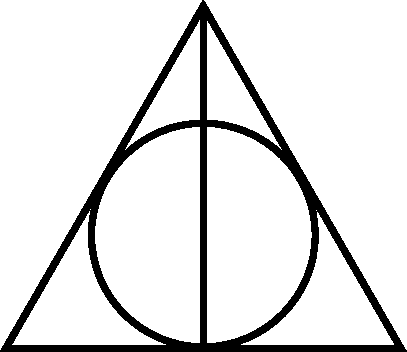
\includegraphics[scale=0.75]{Deathly_Hallows_Sign.pdf}
\end{center}
}
\vspace*{\fill}
\clearpage

%  LocalWords:  nd Kahneman eeeeviiil medi Hmmm stalkery
